
\documentclass[letterpaper,hide notes,xcolor={table,svgnames},pdftex,10pt]{beamer}
\def\showexamples{t}


%\usepackage[svgnames]{xcolor}

%% Demo talk
%\documentclass[letterpaper,notes=show]{beamer}

\usecolortheme{crane}
\setbeamertemplate{navigation symbols}{}

\usetheme{MyPittsburgh}
%\usetheme{Frankfurt}

%\usepackage{tipa}

\usepackage{hyperref}
\usepackage{graphicx,xspace}
\usepackage[normalem]{ulem}
\usepackage{multicol}

\newcommand\SF[1]{$\bigstar$\footnote{SF: #1}}

\usepackage[default]{sourcesanspro}
\usepackage[T1]{fontenc}

\newcounter{tmpnumSlide}
\newcounter{tmpnumNote}

% old question code
%\newcommand\question[1]{{$\bigstar$ \small \onlySlide{2}{#1}}}
% \newcommand\nquestion[1]{\ifdefined \presentationonly \textcircled{?} \fi \note{\par{\Large \textbf{?}} #1}}
% \newcommand\nanswer[1]{\note{\par{\Large \textbf{A}} #1}}


 \newcommand\mnote[1]{%
   \addtocounter{tmpnumSlide}{1}
   \ifdefined\showcues {~\tiny\fbox{\arabic{tmpnumSlide}}}\fi
   \note{\setlength{\parskip}{1ex}\addtocounter{tmpnumNote}{1}\textbf{\Large \arabic{tmpnumNote}:} {#1\par}}}

\newcommand\mmnote[1]{\note{\setlength{\parskip}{1ex}#1\par}}

%\newcommand\mnote[2][]{\ifdefined\handoutwithnotes {~\tiny\fbox{#1}}\fi
% \note{\setlength{\parskip}{1ex}\textbf{\Large #1:} #2\par}}

%\newcommand\mnote[2][]{{\tiny\fbox{#1}} \note{\setlength{\parskip}{1ex}\textbf{\Large #1:} #2\par}}

\newcommand\mquestion[2]{{~\color{red}\fbox{?}}\note{\setlength{\parskip}{1ex}\par{\Large \textbf{?}} #1} \note{\setlength{\parskip}{1ex}\par{\Large \textbf{A}} #2\par}\ifdefined \presentationonly \pause \fi}

\newcommand\blackboard[1]{%
\ifdefined   \showblackboard
  {#1}
  \else {\begin{center} \fbox{\colorbox{blue!30}{%
         \begin{minipage}{.95\linewidth}%
           \hspace{\stretch{1}} Some space intentionally left blank; done at the blackboard.%
         \end{minipage}}}\end{center}}%
         \fi%
}



%\newcommand\q{\tikz \node[thick,color=black,shape=circle]{?};}
%\newcommand\q{\ifdefined \presentationonly \textcircled{?} \fi}

\usepackage{listings}
\lstset{%
  keywordstyle=\bfseries,
  aboveskip=15pt,
  belowskip=15pt,
  captionpos=b,
  identifierstyle=\ttfamily,
  escapeinside={(*@}{@*)},
  stringstyle=\ttfamiliy,
  frame=lines,
  numbers=left, basicstyle=\scriptsize, numberstyle=\tiny, stepnumber=0, numbersep=2pt}

\usepackage{siunitx}
\newcommand\sius[1]{\num[group-separator = {,}]{#1}\si{\micro\second}}
\newcommand\sims[1]{\num[group-separator = {,}]{#1}\si{\milli\second}}
\newcommand\sins[1]{\num[group-separator = {,}]{#1}\si{\nano\second}}
\sisetup{group-separator = {,}, group-digits = true}

%% -------------------- tikz --------------------
\usepackage{tikz}
\usetikzlibrary{positioning}
\usetikzlibrary{arrows,backgrounds,automata,decorations.shapes,decorations.pathmorphing,decorations.markings,decorations.text}

\tikzstyle{place}=[circle,draw=blue!50,fill=blue!20,thick, inner sep=0pt,minimum size=6mm]
\tikzstyle{transition}=[rectangle,draw=black!50,fill=black!20,thick, inner sep=0pt,minimum size=4mm]

\tikzstyle{block}=[rectangle,draw=black, thick, inner sep=5pt]
\tikzstyle{bullet}=[circle,draw=black, fill=black, thin, inner sep=2pt]

\tikzstyle{pre}=[<-,shorten <=1pt,>=stealth',semithick]
\tikzstyle{post}=[->,shorten >=1pt,>=stealth',semithick]
\tikzstyle{bi}=[<->,shorten >=1pt,shorten <=1pt, >=stealth',semithick]

\tikzstyle{mut}=[-,>=stealth',semithick]

\tikzstyle{treereset}=[dashed,->, shorten >=1pt,>=stealth',thin]

\usepackage{ifmtarg}
\usepackage{xifthen}
\makeatletter
% new counter to now which frame it is within the sequence
\newcounter{multiframecounter}
% initialize buffer for previously used frame title
\gdef\lastframetitle{\textit{undefined}}
% new environment for a multi-frame
\newenvironment{multiframe}[1][]{%
\ifthenelse{\isempty{#1}}{%
% if no frame title was set via optional parameter,
% only increase sequence counter by 1
\addtocounter{multiframecounter}{1}%
}{%
% new frame title has been provided, thus
% reset sequence counter to 1 and buffer frame title for later use
\setcounter{multiframecounter}{1}%
\gdef\lastframetitle{#1}%
}%
% start conventional frame environment and
% automatically set frame title followed by sequence counter
\begin{frame}%
\frametitle{\lastframetitle~{\normalfont(\arabic{multiframecounter})}}%
}{%
\end{frame}%
}
\makeatother

\makeatletter
\newdimen\tu@tmpa%
\newdimen\ydiffl%
\newdimen\xdiffl%
\newcommand\ydiff[2]{%
    \coordinate (tmpnamea) at (#1);%
    \coordinate (tmpnameb) at (#2);%
    \pgfextracty{\tu@tmpa}{\pgfpointanchor{tmpnamea}{center}}%
    \pgfextracty{\ydiffl}{\pgfpointanchor{tmpnameb}{center}}%
    \advance\ydiffl by -\tu@tmpa%
}
\newcommand\xdiff[2]{%
    \coordinate (tmpnamea) at (#1);%
    \coordinate (tmpnameb) at (#2);%
    \pgfextractx{\tu@tmpa}{\pgfpointanchor{tmpnamea}{center}}%
    \pgfextractx{\xdiffl}{\pgfpointanchor{tmpnameb}{center}}%
    \advance\xdiffl by -\tu@tmpa%
}
\makeatother
\newcommand{\copyrightbox}[3][r]{%
\begin{tikzpicture}%
\node[inner sep=0pt,minimum size=2em](ciimage){#2};
\usefont{OT1}{phv}{n}{n}\fontsize{4}{4}\selectfont
\ydiff{ciimage.south}{ciimage.north}
\xdiff{ciimage.west}{ciimage.east}
\ifthenelse{\equal{#1}{r}}{%
\node[inner sep=0pt,right=1ex of ciimage.south east,anchor=north west,rotate=90]%
{\raggedleft\color{black!50}\parbox{\the\ydiffl}{\raggedright{}#3}};%
}{%
\ifthenelse{\equal{#1}{l}}{%
\node[inner sep=0pt,right=1ex of ciimage.south west,anchor=south west,rotate=90]%
{\raggedleft\color{black!50}\parbox{\the\ydiffl}{\raggedright{}#3}};%
}{%
\node[inner sep=0pt,below=1ex of ciimage.south west,anchor=north west]%
{\raggedleft\color{black!50}\parbox{\the\xdiffl}{\raggedright{}#3}};%
}
}
\end{tikzpicture}
}


%% --------------------

%\usepackage[excludeor]{everyhook}
%\PushPreHook{par}{\setbox0=\lastbox\llap{MUH}}\box0}

%\vspace*{\stretch{1}

%\setbox0=\lastbox \llap{\textbullet\enskip}\box0}

\setlength{\parskip}{\fill}

\newcommand\noskips{\setlength{\parskip}{1ex}}
\newcommand\doskips{\setlength{\parskip}{\fill}}

\newcommand\xx{\par\vspace*{\stretch{1}}\par}
\newcommand\xxs{\par\vspace*{2ex}\par}
\newcommand\tuple[1]{\langle #1 \rangle}
\newcommand\code[1]{{\sf \footnotesize #1}}
\newcommand\ex[1]{\uline{Example:} \ifdefined \presentationonly \pause \fi
  \ifdefined\showexamples#1\xspace\else{\uline{\hspace*{2cm}}}\fi}

\newcommand\ceil[1]{\lceil #1 \rceil}


\AtBeginSection[]
{
   \begin{frame}
       \frametitle{Outline}
       \tableofcontents[currentsection]
   \end{frame}
}



\pgfdeclarelayer{edgelayer}
\pgfdeclarelayer{nodelayer}
\pgfsetlayers{edgelayer,nodelayer,main}

\tikzstyle{none}=[inner sep=0pt]
\tikzstyle{rn}=[circle,fill=Red,draw=Black,line width=0.8 pt]
\tikzstyle{gn}=[circle,fill=Lime,draw=Black,line width=0.8 pt]
\tikzstyle{yn}=[circle,fill=Yellow,draw=Black,line width=0.8 pt]
\tikzstyle{empty}=[circle,fill=White,draw=Black]
\tikzstyle{bw} = [rectangle, draw, fill=blue!20, 
    text width=4em, text centered, rounded corners, minimum height=2em]
    
    \newcommand{\CcNote}[1]{% longname
	This work is licensed under the \textit{Creative Commons #1 3.0 License}.%
}
\newcommand{\CcImageBy}[1]{%
	\includegraphics[scale=#1]{creative_commons/cc_by_30.pdf}%
}
\newcommand{\CcImageSa}[1]{%
	\includegraphics[scale=#1]{creative_commons/cc_sa_30.pdf}%
}
\newcommand{\CcImageNc}[1]{%
	\includegraphics[scale=#1]{creative_commons/cc_nc_30.pdf}%
}
\newcommand{\CcGroupBySa}[2]{% zoom, gap
	\CcImageBy{#1}\hspace*{#2}\CcImageNc{#1}\hspace*{#2}\CcImageSa{#1}%
}
\newcommand{\CcLongnameByNcSa}{Attribution-NonCommercial-ShareAlike}

\newenvironment{changemargin}[1]{% 
  \begin{list}{}{% 
    \setlength{\topsep}{0pt}% 
    \setlength{\leftmargin}{#1}% 
    \setlength{\rightmargin}{1em}
    \setlength{\listparindent}{\parindent}% 
    \setlength{\itemindent}{\parindent}% 
    \setlength{\parsep}{\parskip}% 
  }% 
  \item[]}{\end{list}} 




\title{Lecture 12 --- Tort: Introduction }

\author{Jeff Zarnett \\ \small \texttt{jzarnett@uwaterloo.ca}}
\institute{Department of Electrical and Computer Engineering \\
  University of Waterloo}
\date{\today}


\begin{document}

\begin{frame}
  \titlepage

\begin{center}
  \small{Acknowledgments: Douglas Harder~\cite{dwh}, Julie Vale~\cite{jv}}
  \end{center}
\end{frame}




\begin{frame}
\frametitle{The Cake is a Lie}

The next major area of law is \alert{tort} law.

\begin{center}
	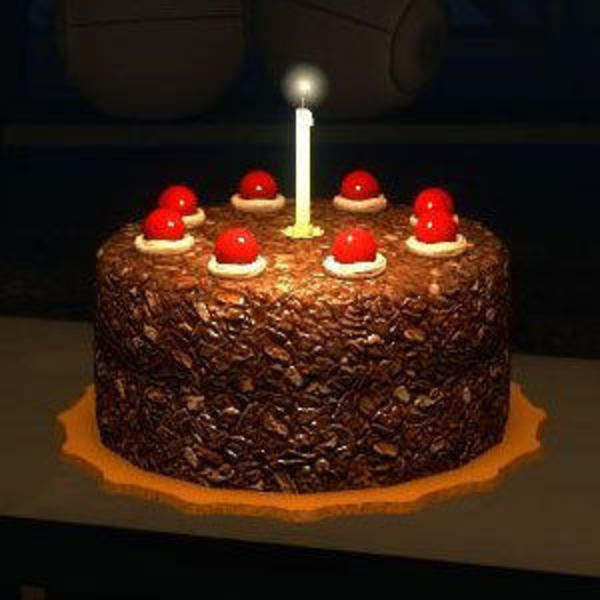
\includegraphics[width=0.3\textwidth]{images/portal-cake.jpg}
\end{center}

Not to be confused with \textit{torte} (cake).

Tort (from the medieval latin word for ``wrong'') is the action of causing harm to another person.


\end{frame}



\begin{frame}
\frametitle{Torts}

The key idea of tort law is in the idea of a harm suffered by someone. 

The basic issue is: who shall bear the loss~\cite{lba}?\\
\quad The victim? The perpetrator? An insurance company? Society as a whole?

The primary purpose of tort law is not to punish wrongdoers, but instead to compensate those who are wronged.

Punishment, if necessary, is usually left to the criminal law system.

\end{frame}



\begin{frame}
\frametitle{Crime and Punishment}

A small digression on crime and punishment. 

A breach of a statute, an act of parliament, is called an \alert{offence}.

Offences listed in the Criminal Code of Canada merit special attention because conviction of a criminal offence results in a sentence and criminal record.

Other offences do not result in this record; once punishment is dispensed that is the end of the matter.

In either case, the penalty is a punishment and will hopefully deter would-be offenders and hopefully rehabilitate those who have offended.

Remember, however, that a crime is an offence against the state.

\end{frame}



\begin{frame}
\frametitle{Private Persons}

When a person causes harm to another, the harm may not have broken a law or a contract, but nevertheless, a person has been harmed.

The injured party may be able to seek compensation through tort law.

The two parties are referred to as the \alert{tortfeasor} (wrongdoer) and \alert{victim}.

Normally the victim can apply to the court for compensation resulting from the harm caused. The victim will need to show damages.

Keep in mind that a corporation or other form of business organization is a ``legal person'' (not a ``natural person'') and can be a party in tort law.

\end{frame}



\begin{frame}
\frametitle{Punitive Damages}

Under rare circumstances the court will award \alert{punitive damages}.\\
\quad This is another way of punishing the tortfeasor.

There are a number of arguments for and against punitive damages...\\
\quad For discussion: what arguments might you make?

Usually they will be awarded only in cases where the tortfeasor's behaviour was especially egregious, malicious, intentional, etc...

\end{frame}



\begin{frame}
\frametitle{Development of the Tort Concept}

In the early days of tort law, it was very simple: anyone who caused a violent injury to another had to pay~\cite{lba}.

A man is walking down the road and trampled by a horse loose from a carriage.

Under the old system, the owner of the horse or operator of the carriage is responsible, period, end of story.

Over time, this concept was refined to include the idea of \alert{fault}. 

So if he was careless and let the horse escape for that reason, the operator is still liable and must pay.

But if the horse was scared by a snake, that is beyond the operator's control, and he will not be considered liable.

\end{frame}



\begin{frame}
\frametitle{Development of the Tort Concept}

The definition of tort was also expanded to include less direct situations~\cite{lba}.


Suppose A carelessly drops a log on the road at sunset and leaves it there.

B's horde trips over the log and is injured.

In early law, this was not recognized as being ``A's fault''.

Later, the court's recognized that A's action (inaction) was responsible for B's injury, indirectly, and this allowed B to recover damages.

So now the law accounts for both fault and \alert{causation}.

\end{frame}


\begin{frame}
\frametitle{Elements of Tort Action}

To establish the right to recover compensation, the plaintiff must prove~\cite{lpe}:

\begin{enumerate}
	\item The defendant owed the plaintiff a duty of care
	\item The defendant breached that duty by his or her conduct
	\item The defendant's conduct caused the injury to the plaintiff
\end{enumerate}

If any one of those elements is absent, the action will fail.

\end{frame}



\begin{frame}
\frametitle{Duty of Care}

\alert{Duty of Care}: a duty that a person has to ensure that others do not suffer a harm or loss.

A duty typically arises when a person takes an action that could reasonably harm others, such as driving or providing engineering consulting services.

\alert{Reasonableness} is a very large element of tort law. 

The courts will usually hold parties to the standard of ``the conduct expected of a reasonable person under the circumstances''~\cite{lpe}.

\end{frame}



\begin{frame}
\frametitle{Causation}

The third element in the list requires the plaintiff to establish causation.

Example~\cite{lba}: Suppose that Alice breaks a plate on Monday at dinner time.

The next day, her wife Beth makes a special trip by car to a shop to replace it.

On her way she gets in a car crash.

Is Alice's carelessness in dropping the plate responsible for the car accident?

\end{frame}



\begin{frame}
\frametitle{Causation}

In the eyes of the law, Alice did not cause the accident.

It is true that had Alice not dropped the plate, Beth would not have been on her way to the store, and not have been in the crash.

However, many voluntary acts intervened between the dropping of the plate.

Beth could have chosen to go at another time, as the other driver might have.

These voluntary acts ``decouple'' the two events.\\
\quad Causation can be traced back to the voluntary acts but no further.

\end{frame}



\begin{frame}
\frametitle{Causation}

Another idea: the car crash may have occurred due to carelessness on the part of Beth or the other driver.

Had they driven carefully, no collision would have occurred.

Here, the careless conduct may also ``decouple'' the events.\\
\quad Causation can be traced back to the careless acts but no further.

\end{frame}



\begin{frame}
\frametitle{Causation}

As a general rule, the closer a person's conduct is to the event in question, the less chance there is of an intervening event~\cite{lba}.

Imagine that Charles makes a sudden, unsafe left turn and Darryl makes an unwise decision and crashes into him. 

The suddenness of Charles's action makes him the ``cause'' of the collision. 

And if Charles made that move five seconds earlier, giving Darryl additional time to make a decision to avoid the collision? 

Then we may find that Darryl is responsible because he could have avoided the collision but did not.

\end{frame}



\begin{frame}
\frametitle{Burden of Proof}

The burden of proof in tort law cases is somewhat complex~\cite{lba}.

Suppose that Eve gets sick because of a poisonous substance in a can of tuna that she purchases.

She may be able to establish that there was poison in the can, but it would be very difficult for her to find out how it happened.

In tort law, the injured party need only demonstrate the defendant's product caused the injury; not the exact details of how.

Then the defendant must prove that they are not responsible for the injury.\\
\quad The burden has shifted to the defendant in that case.


\end{frame}



\begin{frame}
\frametitle{Intentional Torts}

Tort can be classified based on intent.

An \alert{intentional tort} is one where the tortfeasor deliberately performs an action which harms another.

For the most part in this course we will focus on \alert{unintentional torts}.

Still, we will briefly examine the intentional torts.

\end{frame}



\begin{frame}
\frametitle{Intentional Torts}

The intentional torts we will discuss are:

\begin{itemize}
	\item Trespassing 
	\item Nuisance
	\item Defamation
	\item Fraud
	\item Assault
	\item Battery
	\item Invasion of Privacy
	\item Intentional Infliction of Emotional Distress
	\item False Arrest/Imprisonment
	\item Conversion
\end{itemize}

Basically: don't do any of these things!

\end{frame}



\begin{frame}
\frametitle{Trespassing}

Trespassing is probably a tort with which everyone is vaguely familiar.

It is entering the property of another without permission, or refusal to leave after being asked to do so by the owner.

The owner of the property may use no more than reasonable force in ejecting a trespasser~\cite{lba}.

The owner of property is unlikely to recover more than nominal damages unless it can be demonstrated that the trespasser caused harm to the property...

\end{frame}



\begin{frame}
\frametitle{Nuisance}

A person has a right to enjoy his or her real property (land) and when another interferes with that enjoyment, the second party is guilty of the tort of nuisance.

Examples include loud music, trash fires, pollution, etc.

The harm might be simply that noise or smell prevents the owner from enjoying his/her property, or it could be actual damage.

Discussion: how might reasonableness apply here?

\end{frame}


\begin{frame}
\frametitle{Defamation}

Defamation occurs when untrue statements damage someone's reputation.\\
\quad It must be conveyed to a third party (just insulting someone is not enough).

Note that they must be untrue. If the statement is factually correct then it is not a tort, no matter how damaging it is to a person's reputation.

Defamation is usually broken down into \alert{slander} (the spoken form) or \alert{libel} (the written form).

It must be an attack on the victim's actual representation, not just the reputation they think they deserve.

\end{frame}

\begin{frame}
\frametitle{Fraud}

Fraud is a criminal act and this may be prosecuted separately by the crown.

However, that is criminal punishment and the defrauded party can seek recourse from the civil justice system.

The victim of fraud can then recover damages as a after having been defrauded.

\end{frame}



\begin{frame}
\frametitle{Assault \& Battery}

These two often go together, but are separate.

Assault:\\
\begin{itemize}
	\item Threat to commit unwanted physical contact
	\item Reasonable belief to feel threatened
\end{itemize}

Assault can also be a criminal offence.

Battery:\\
\begin{itemize}
	\item Unwanted direct or indirect contact
	\item Contact was intentional
\end{itemize}

Battery is sometimes referred to as a trespass to the person.

\end{frame}



\begin{frame}
\frametitle{Invasion of Privacy}

In 2012 Ontario recognized the tort of Invasion of Privacy in \textit{Jones v. Tsige}.

This is also called ``intrusion upon seclusion''.

The defendant committed the invasion of privacy when she used her position as a bank employee to look at the private banking records of her spouse's ex-wife.

\end{frame}



\begin{frame}
\frametitle{Intentional Infliction of Emotional Distress}

This tort is not about hurt feelings, but it does require that the tortfeasor actually cause serious distress.

It must be flagrant or outrageous conduct, calculated to produce harm, resulting in a visible illness. 

This can come up when an employer acts in an unreasonable way to try to force an employee to quit. 

Someone harassing or stalking an ex-partner may commit this tort.


\end{frame}



\begin{frame}
\frametitle{False Arrest/Imprisonment}

False Arrest and False Imprisonment are separate but very similar.

The important thing is that the victim is wrongfully deprived of liberty.

False arrest requires an insufficient reason to arrest or excessive force.

False imprisonment requires a lack of lawful authority.


\end{frame}



\begin{frame}
\frametitle{Conversion}

Conversion is about making use of another's property without the consent of the owner.

Taking, using, or destroying goods that belongs to others.

This must also have the effect or intention of interfering with or denying the victim's rights to the property.


\end{frame}


\begin{frame}
\frametitle{References \& Disclaimer}
\bibliographystyle{alphaurl}
\setbeamertemplate{bibliography item}{\insertbiblabel}
{\scriptsize
\bibliography{290}
}
\vfill

{\tiny Disclaimer: the material presented in these lectures slides is intended for use in the course ECE~290 at the University of Waterloo and should not be relied upon as legal advice. Any reliance on these course slides by any party for any other purpose are the responsibility of such parties.  The author(s) accept(s) no responsibility for damages, if any, suffered by any party as a result of decisions made or actions based on these course slides for any other purpose than that for which it was intended.\par}


\end{frame}


\end{document}

